\documentclass[a4paper]{article}
\usepackage[utf8]{inputenc}
\usepackage{authblk}
\usepackage{graphicx}
\usepackage{color}
\usepackage{verbatim}
\usepackage{enumerate}
\usepackage{multicol}
\usepackage{multirow}

\usepackage{amsmath}


\title{CSE 300: Online Assignment}
\author[1,*]{Md Shamsuzzoha Bayzid}
\author[1,\dagger{}] { Mahjabin Nahar}
\author[1,\dagger{}] {Md Shariful Islam Bhuyan}
\author[1,\dagger{}] {Md Saidur Rahman}

\affil[1]{Department of Computer Science and Engineering   Bangladesh University of Engineering and Technology}
\affil[*]{Corresponding author: shams\_bayzid@cse.buet.ac.bd}
\affil[\dagger{}]{These authors contributed equally to this work}

\date{April 07, 2021}


\begin{document}

\maketitle


\section{Introduction}
This assignment has been designed to assess the preparation of the students in writing
scientific articles using \LaTeX{}. Different components, that are frequently used in scientific
manuscripts, have been covered in this assignment.

\subsection{Tables}
We wish to place Table \ref{tab:table1} right here.

\begin{table}[h]
    \centering
    \caption{\textbf{Optimization scores for Method-1 and Method-2 on different datasets
covering various model conditions.} We show average scores of two optimization
criteria for various model conditions}
    \begin{tabular}{|c|cc|cc|cc|}
         \hline
         \multicolumn{3}{|c|}{Simulation Condition} & \multicolumn{4}{|c|}{Optimization Score} \\
         \hline
         \multirow{2}{*}{Dataset} & \multirow{2}{*}{Complexity} & Model & \multicolumn{2}{|c|}{Score 1} &  \multicolumn{2}{|c|}{Score 2} \\
         \cline{4-7}
         & & condition & Method-1 & Method-2 & Method-1 & Method-2 \\
         \hline
         \hline
         \multirow{4}{*}{D1} & \multirow{2}{*}{Easy} & M_1 & 7,425.55 & 770.00 & 929.55 & 10 \\
         & & M_2 & 7,657.00 & 9,179.00 & 716.15 & 20 \\
         \cline{2-7}
         & \multirow{2}{*}{Hard} & M_3 & 54.00 & 9,007.15 & 3,759.00 & 30 \\
         & & M_4 & 74.00 & 5567.15 & 99.00 & 25 \\
         \hline
         \hline
         \multirow{3}{*}{D3} & \multirow{3}{*}{Moderate} & M_1 & 34.00 & 273.00 & 321.60 & 34 \\
         & & M_2 & \multicolumn{2}{|c|}{Not Applicable} & 16.00  & 11 \\
         & & M_3 & 657.00 & 179.60 & 716.00 & 19 \\
         \hline
    \end{tabular}
    
    \label{tab:table1}
\end{table}
\pagebreak
\begin{figure}[t]
    \centering
    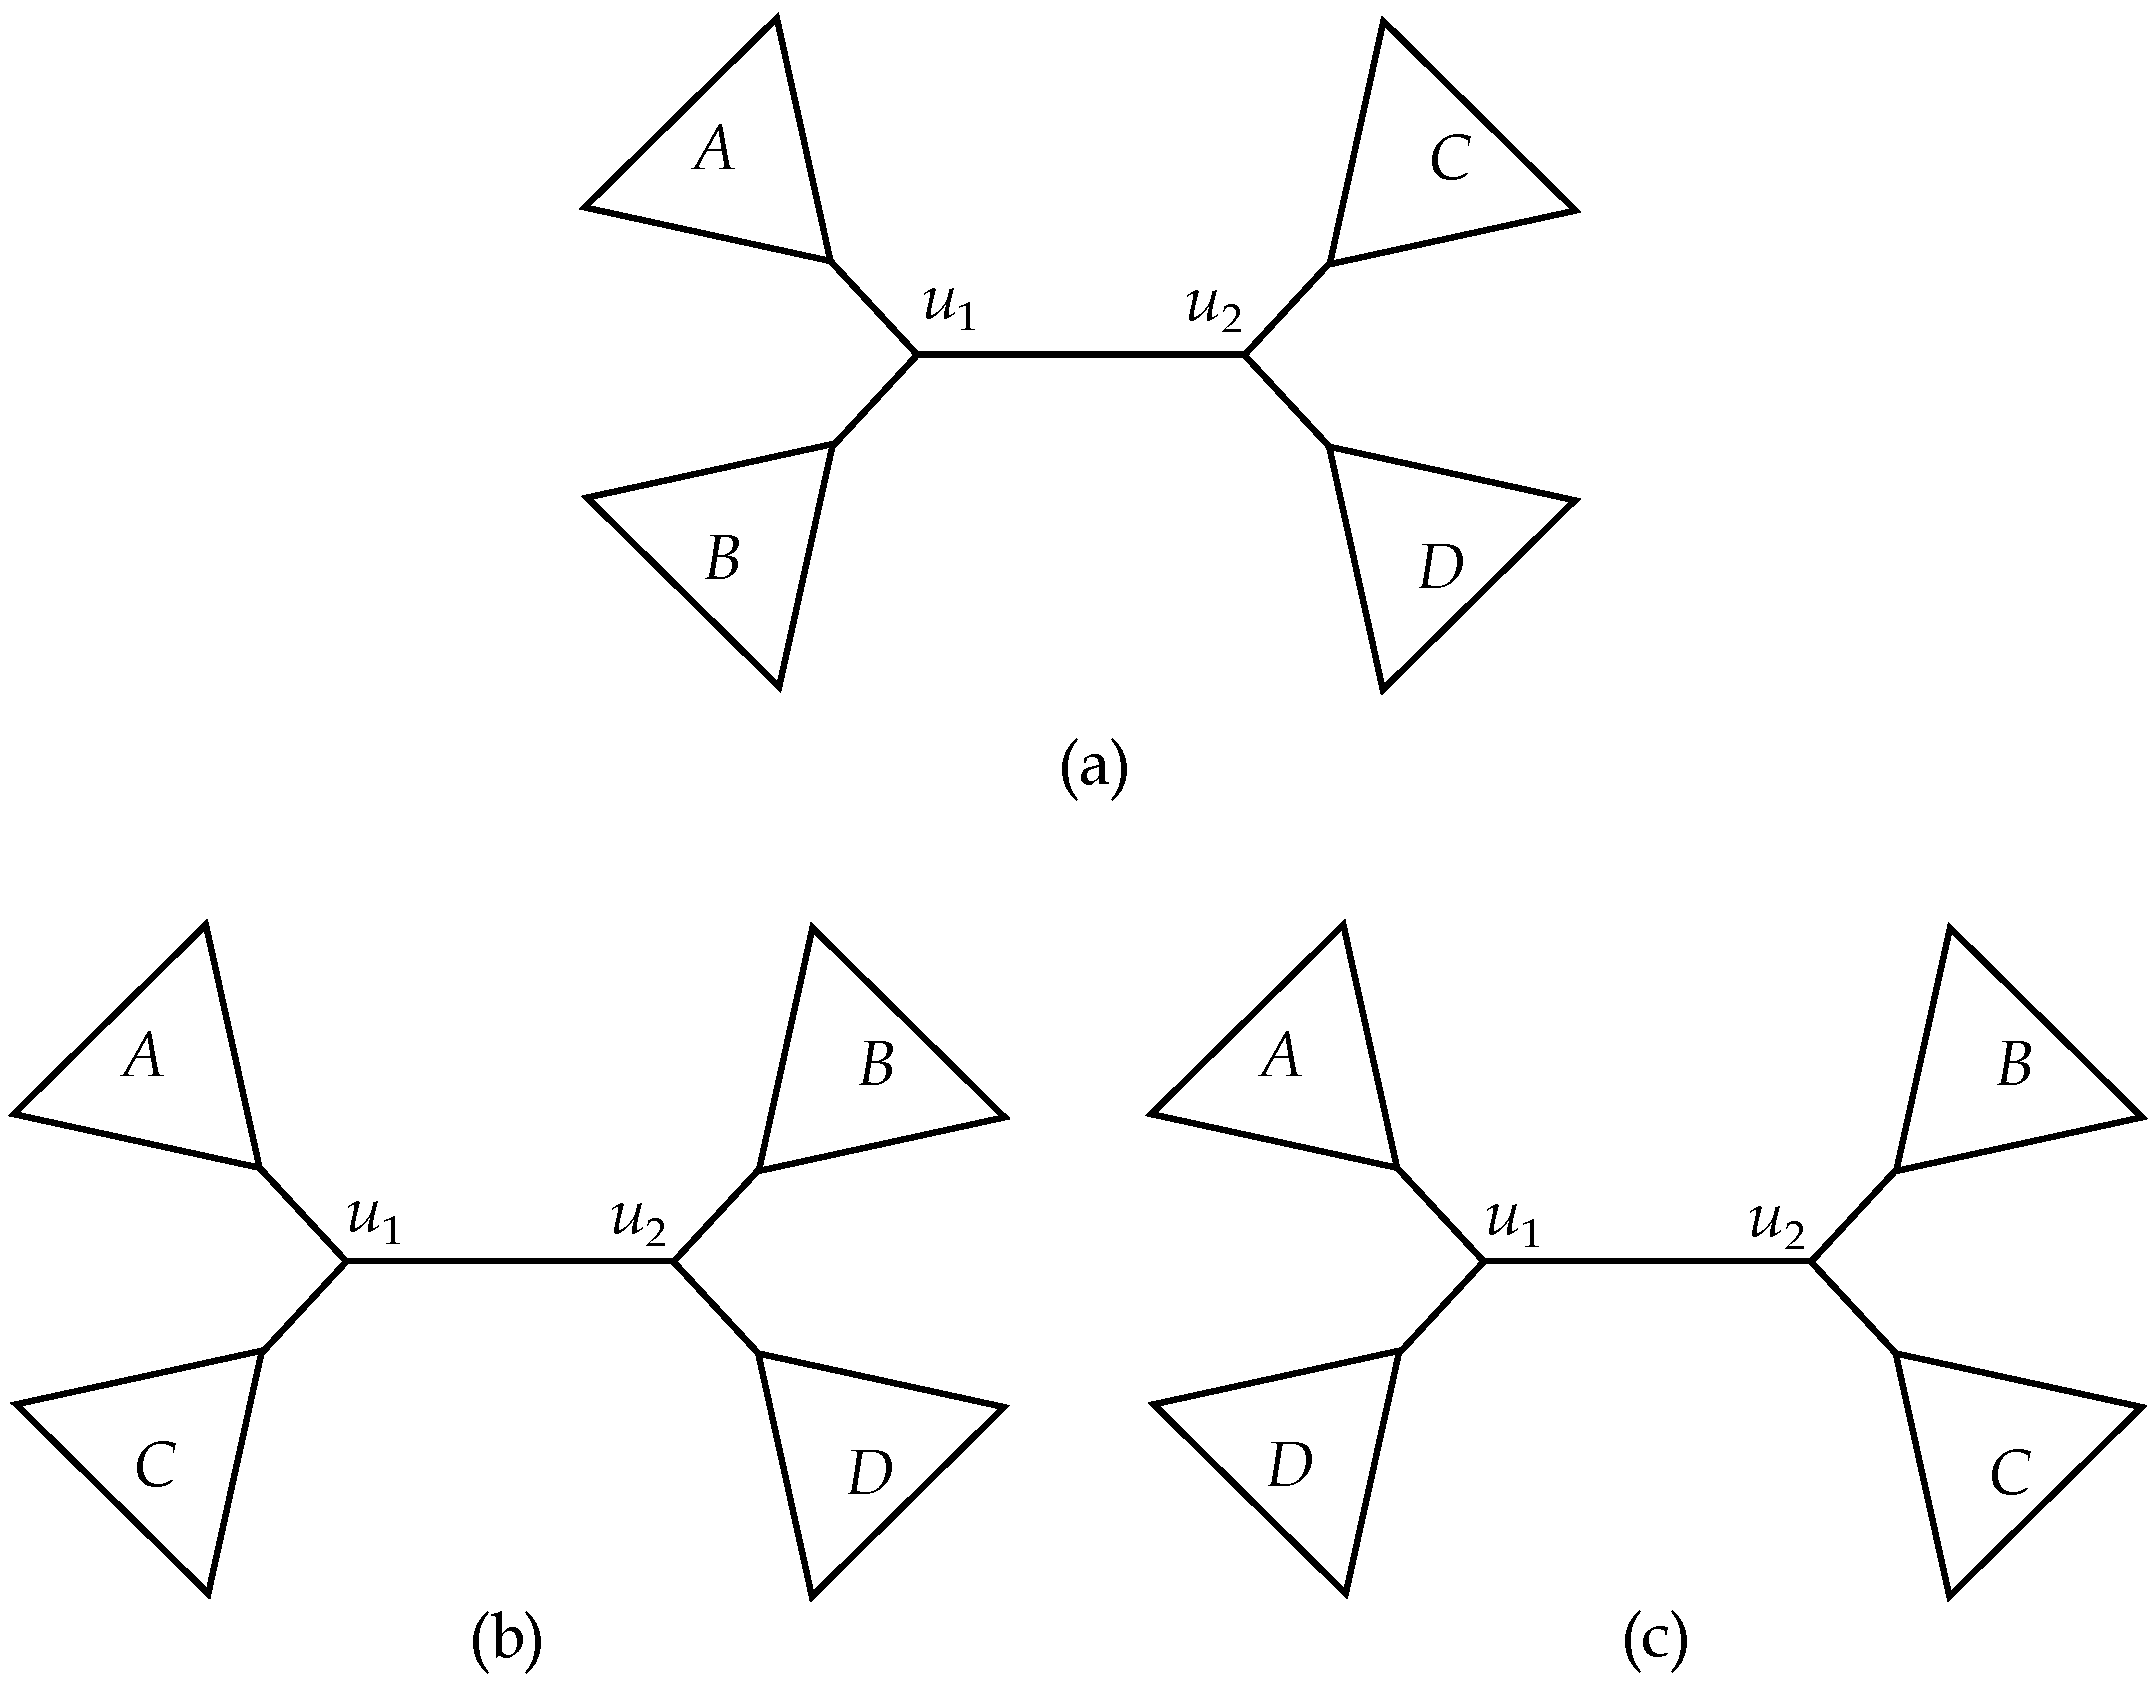
\includegraphics[width=.7\textwidth]{Figure3}
    \caption{ \textbf{Nearest Neighbor Interchange (NNI) move on an internal edge.} (a)
A species tree ST, and (b)-(c) the neighbors of ST resulting from one NNI move on edge
$e = (u1, u2)$. A, B, C, and D are the sets of taxa in the four subtrees around edge $e$.}
    \label{fig:fig1}
\end{figure}

\subsection{Figures}
We intend to put Figure \ref{fig:fig1} at the top of a page.

\subsection{Equations}
Let n1\textbar n2\textbar n3 be a tripartition defined on an internal node $u$ of a binary tree $T$. The
number of tripartitions mapped to u is given by Eqn. \ref{eqn: e1}
\begin{align}
      $\mathcal{NQ}$(n_1,n_2,n_3) & = \binom{n_1}{2} \binom{n_2}{1} \binom{n_3}{1} + \binom{n_2}{2} \binom{n_1}{1} \binom{n_3}{1} + \binom{n_3}{2} \binom{n_1}{1} \binom{n_2}{1} \\
   & = \frac{n_1n_2n_3(n_1 + n_2 + n_3 - 3)}{2} 
   \label{eqn: e1}
\end{align}
\section{Conclusions}
The major objectives of this assignment are listed below (please do not ignore the font
sizes). \\
\begin{itemize}
    \item \Large{ To see if the students have adequately practiced different aspects of writing in \LaTeX{}.}
    \item \large{To assess the ability of the students in preparing manuscripts in \LaTeX{}.}
    \item \small{To see if the students can add various basic components (e.g., tables, figures, equations) to a \LaTeX{} manuscript}
    \item To see if the students can leverage the available materials (both offline and online) to do
something which has not explicitly been taught in the class.
\end{itemize}

\end{document}